\documentclass{article}

\usepackage{graphicx}
\usepackage{hyperref}
\usepackage{amsmath}
\usepackage{amssymb}
\usepackage{blkarray}
\usepackage{cancel}
\usepackage{fancyhdr}
\usepackage{enumitem}
\usepackage{lscape}
\usepackage{listings}
\usepackage{color}
\usepackage{pdfpages}
\usepackage{yfonts}
\usepackage{caption}
\usepackage{natbib}
\definecolor{dkgreen}{rgb}{0,0.6,0}
\definecolor{gray}{rgb}{0.5,0.5,0.5}
\definecolor{mauve}{rgb}{0.58,0,0.82}
\usepackage[toc,page]{appendix}

\usepackage{xcolor}

\lstdefinestyle{base}{
  inputencoding=latin10,
  emptylines=1,
  breaklines=true,
  basicstyle=\small\ttfamily,
  moredelim=**[is][\color{red}]{@}{@},
}

\newcommand{\norm}[1]{\left\lVert#1\right\rVert}

%% Define a HUGE 
\makeatletter
\newcommand\HUGE{\@setfontsize\Huge{50}{60}}
\makeatother

\begin{document}             % End of preamble and beginning of text.

 
%titlepage
\thispagestyle{empty}
\begin{center}
\begin{minipage}{.9\linewidth}
\flushright
	      		 

\includegraphics[width=0.5\linewidth]{univie.eps}\par
\vspace{1.5cm}
\centering 	
    % Title
	{\scshape{\HUGE A5 Report \par}}
	\vspace{1cm}
	%Thesis title
    {\scshape{\Large Course: VIS WS '18/19 \quad  date: 23.01.2019\par}}
	\vspace{1cm}

 {\Large Name : Robert Ernstbrunner \\ Matnr.: 01403753 \hspace{2.2cm} \ \par}
 	\vspace{.7cm}

 

\end{minipage}
\end{center}
\clearpage

\section{Motivation}

The ornithology student Mitch Vogel (yes, he's \textit{still} a birdwatcher named \textit{Vogel}) needs our help in visualizing his data in order to advance in his investigations. There is an observed decline in the nesting \textit{Rose-crested Blue Pipit} in the \textit{Boonsong Lekagul Nature Preserve} and Mitch thinks the traffic going through the preserve might have to do with it.
He reckons that traffic noise might overshadow mating calls or that invading campers might scare away the birds from their habitat areas. \\
The data was collected by park rangers who work as caretakers of the nature preserve. They gave Mitch additional explanations about the data together with a map.\\

I chose the third design from \textit{A4} (Figure~\ref{fig:prototype}, for a detailed description see~\nameref{appendix:a}) mainly because I think it creates the least problems to run into. Tableau can easily handle stream graphs, histograms and stacked barplots. The other designs featured a flow map and parallel coordinates. Both are especially hard to realize in Tableau. However, I could not avoid problems completely and had to slightly alter my design eventually as I will explain in section~\ref{sec:protoimpl}. Of course there are other reasons  that are in favor of this visualization. E.g., the design would not only work for a single day, but also over longer periods of time, since all visualization types are capable of displaying large amounts of data as well and it's nice to have this kind of flexibility.

\begin{figure}[h]
	\centering
	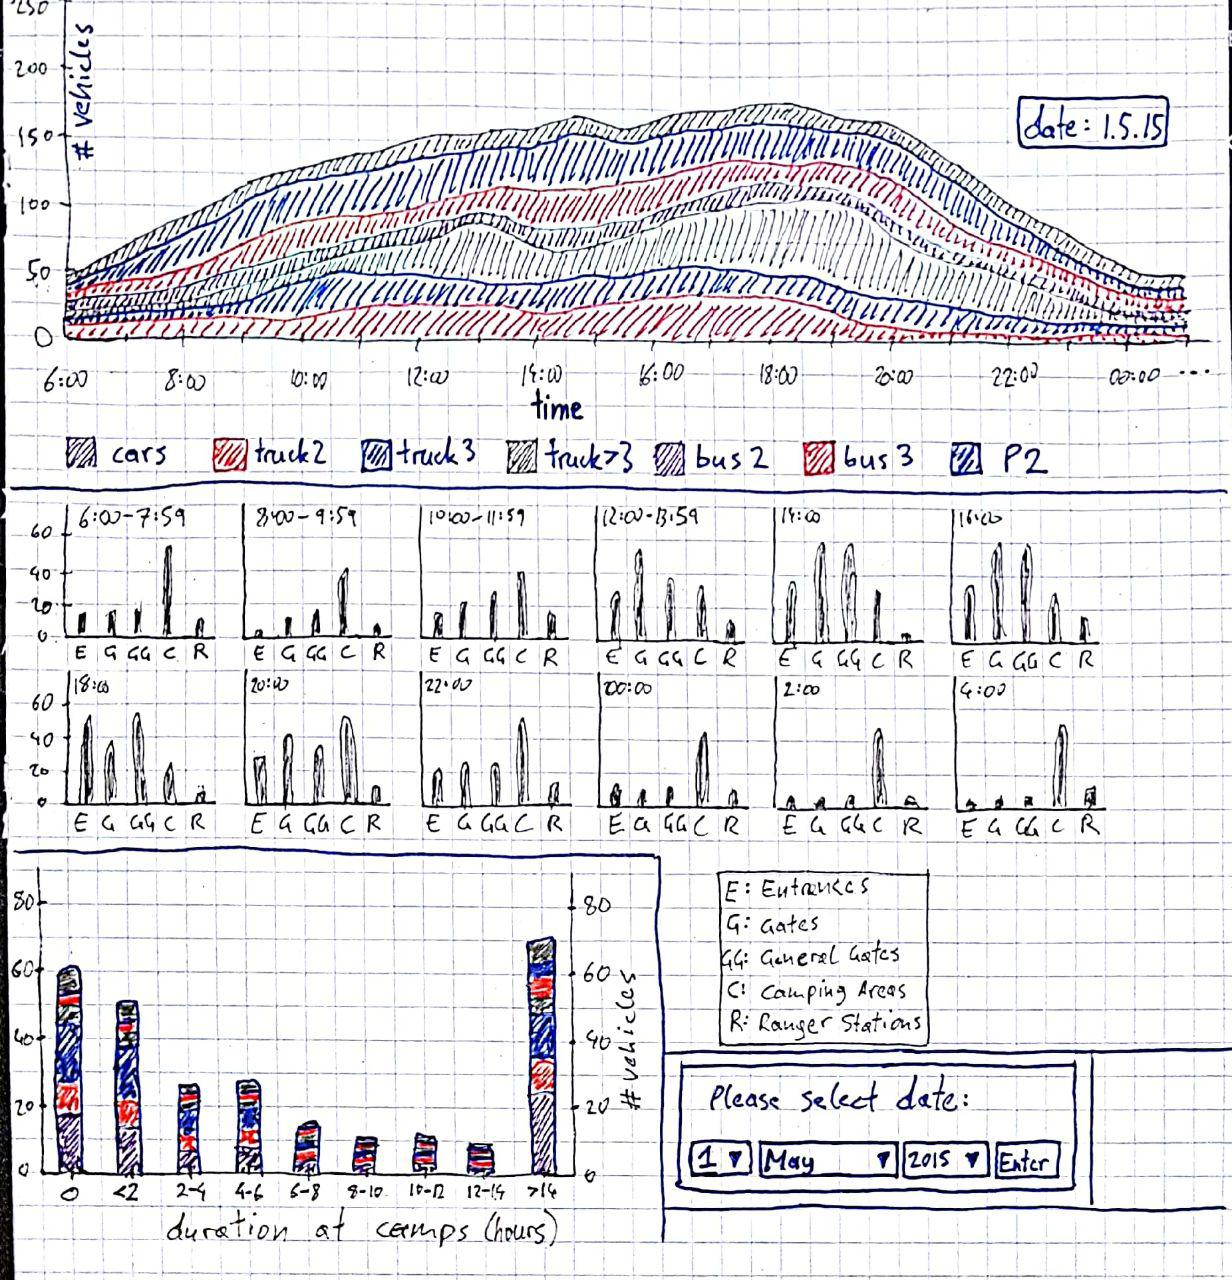
\includegraphics[scale = .45]{Design3.jpg}
	\caption{Design 3 paper prototype}
	\label{fig:prototype}
\end{figure}

\section{Prototype Implementation} \label{sec:protoimpl}
Prototyping the stream graph was rather quick. I over-complicated things at first but was surprised how easily this could be done.
The histograms were a bit tricky. I had to learn how to group by gates and time and had to figure out a way to create two rows of histograms. I ended up hard coding the labels and groupings, which took some time. Therefore, making minor changes to these views might be a time consuming process as well.
Prototyping the stacked barplot was easy again, because I simply switched the duration scale for the time scale. This is where I ran into problems eventually. Transforming the \textit{time} scale into an actual \textit{duration} scale for the final implementation was not manageable in the given amount of time. I tried some things with the \textit{LOOKUP} command and eventually figured, that calculating the duration at camps is a complex process that might be done outside of Tableau instead. Consider, for each vehicle we would have to calculate the difference between the first \textit{camp timestamp} and the consecutive \textit{non-camp timestamp} and sum up multiple occurrences per day. Given my current level of experience with Tableau (beginner) compared to $D3$ (intermediate), preprocessing the data in that way is a task I'd rather do in $D3$ instead.

\section*{Final design}
By and large, my final implementation marginally differs from the paper prototype (see Figure~\ref{fig:tableau}). For reasons explained in the previous section, I had to switch the duration scale for a simpler time scale which is unfortunate, since \textit{Mitch} might have gained more insight if the duration at camps was displayed instead. However, combining the different views and connecting them to the day selector was surprisingly easy to do. Since the prototype was adapted into the final implementation, there is no initial prototype anymore.

\section*{Final implementation}

\begin{figure}[h]
	\centering
	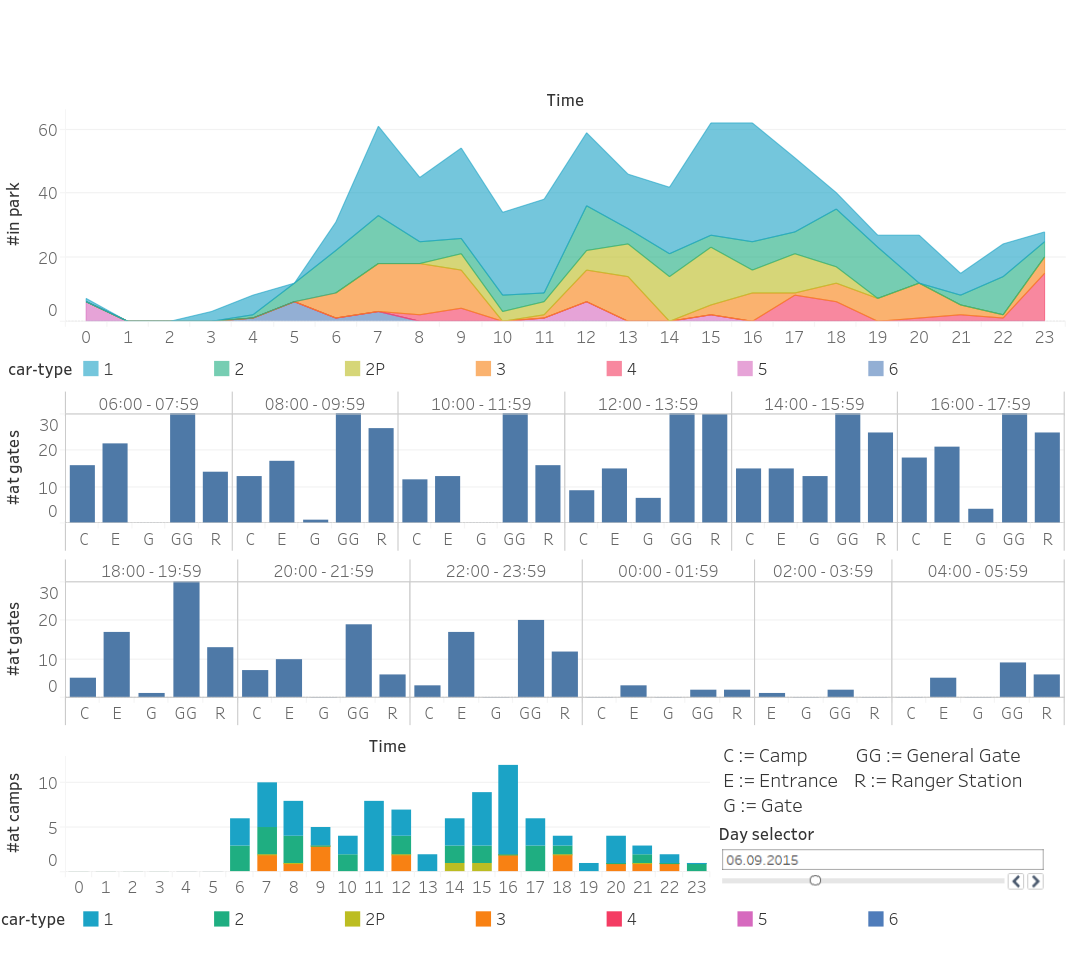
\includegraphics[scale = .53]{tableau_design3.png}
	\caption{Design 3 in Tableau}
	\label{fig:tableau}
\end{figure}

What I could extract from the data is, that during the summer increased traffic and camping could be detected. This suggests that people mostly come for camping. During the off-season the campers, as well as the traffic is reduced and there are mainly rangers who visit camps and trucks that pass through. However, one could not see how long rangers and trucks spent at camps so it isn't clear if they are residing or just passing. Also the car-types are more cars and motorcycles during the summer and mainly trucks during the winter. During the summer the number of vehicles in the park starts to rise at around 6 a.m. and declines around 7 p.m..

\section{Summary}
My final implementation could be improved by adding a brush filter in order to enable views over larger periods of time. This would not be hard to do (e.g. have two selectors for start- and end-time and transform the \textit{day filter} in Tableau to a \textit{between-dates} filter).
What I wonder about is that, during the night, the number of campers is often zero suggesting that no one is resting at night and driving around instead. I think it is more likely that there is some error in the calculations. This necessitates taking a closer look at the raw data. However, I think if this error (if it is one) could be fixed, \textit{Mitch} can definitely gather some valuable information from my visualization. From an implementation point of view I would generate a single day filter for all views instead of writing the filter for each individual view in the individual calculation tables. However I ran into some problems for the steam graph when applying the filter afterwards instead of directly writing it in the table calculation which justifies the individual filters somehow. Also, in the assignment description, it was not quite clear to me what a \textit{Tableau notebook} is. I exported a  packaged Workbook (.twbx File) instead.

\bibliographystyle{plain}
\bibliography{a01403753_A5}


\begin{appendices}
\section*{Appendix A} \label{appendix:a}
\paragraph{Design 3}
For my last design (\texttt{\hyperref[fig:design3]{Figure~\ref{fig:prototype}}}) I chose to work mainly with stacked visualization types to visualize traffic density. The stream graph shows the amount of vehicles that are in the preserve over one day. Since the amount of vehicles is \textit{quantitative} data, and the vehicles themselves are \textit{nominal} and few (i.e. \textit{colorable}) and time is an \textit{ordinal} attribute, this type of visualization was a perfect choice in my opinion\citep{munzner2015visualization}. The day can also be selected with the date selector in the bottom right corner of the design.\\
Below the stream graph I wanted to show movement between the different sensor types. Therefore, I drew histograms at different points in time that show the amount of vehicles currently present at each sensor type. This could have probably been animated as well, but I consider my approach to be superior over animation because the change in the five histogram bars would be too much to comprehend in an animation. Generally, in such cases, the amount of frames should always be reduced, i.e. convert from animation to side-by-side views. In total, there are twelve views distributed over two rows. It was of very importance to me that the views are row-aligned in order to be closer together. This should reduce cognitive load and there is only one line jump were \textit{Mitch} has to rely on his memory instead\citep{munzner2015visualization}. Everyone understanding the english language tends to read from left to right. This habit should also adapt to the side-by-side view.\\
Another thing that might interest \textit{Mitch} is the duration that vehicles spend at camping areas. Since the vehicle types are nominal and colorable,  the duration intervals are nominal and the amount of vehicles is quantitative, it made sense to create a stacked bar chart here\citep{munzner2015visualization}.

\end{appendices}


\end{document}